%
% File ijcnlp2011.tex
%
% Contact  sudeshna@cse.iitkgp.ernet.in
%%
%% Based on the style files for ACL-IJCNLP-2009...

%% Based on the style files for EACL 2006 by
%%e.agirre@ehu.es or Sergi.Balari@uab.es
%% and that of ACL 08 by Joakim Nivre and Noah Smith

\documentclass[10pt]{article}
\usepackage{ijcnlp2011}
\usepackage{times}
\usepackage{url}
\usepackage{amssymb}
\usepackage{latexsym, amsmath}
%\setlength\titlebox{6.5cm}    % You can expand the title box if you
% really have to

\usepackage{epsf, graphicx, subfig, booktabs, alltt, multirow} 
\usepackage{algorithm, algorithmic}
\usepackage[multiple, para]{footmisc}

\DeclareMathOperator*{\argmax}{arg\,max}


\title{TriS: A Statistical Sentence Simplifier \\with Log-linear Models and Margin-based Discriminative Training}

%\author{Nguyen Bach, Qin Gao \and Stephan Vogel \\
%  Language Technologies Institute\\
%  Carnegie Mellon University\\
%  5000 Forbes Avenue, Pittsburgh PA, 15213\\
%  {\tt \{nbach, qing, stephan.vogel\}@cs.cmu.edu}}
%} 

\date{}

\begin{document}
\maketitle
\begin{abstract}

We propose a statistical sentence simplification system with log-linear models. 
In contrast to state-of-the-art methods that drive sentence simplification process by hand-written linguistic rules, our method used a margin-based discriminative learning algorithm operates on a feature set. 
The feature set is defined on statistics of surface form as well as syntactic and dependency structures of the sentences. 
A stack decoding algorithm is used which allows us to efficiently generate and search simplification hypotheses. 
Experimental results show that the simplified text produced by the proposed system reduces 1.7 Flesch-Kincaid grade level when compared with the original text. 
We will show that a comparison of a state-of-the-art rule-based system \cite{HeilmanSmith:2010} to the proposed system demonstrates an improvement of 0.2, 0.6, and 4.5 points in ROUGE-2, ROUGE-4, and $AveF_{10}$, respectively.

%We propose a sentence simplification system with log-linear models. 
%The proposed system uses a stack decoding algorithm which allows us to efficiently generate and search simplification hypotheses based on objects. 
%We also present a margin-based discriminative learning algorithm coupled with a novel feature set defined on surface sentence statistics as well as deep syntactic and dependency structures.
%This differs from current state-of-the-art models that drive sentence simplification process by hand-written linguistic rules. 
%Experimental results show that the proposed system reduces 1.7 Flesch-Kincaid grade level when comparing between the original text and simplified text.
%We will show that a comparison of a state-of-the-art rule-based system \cite{HeilmanSmith:2010} to the proposed system demonstrates an improvement of 0.2, 0.6, and 4.5 points in ROUGE-2, ROUGE-4 and $AveF_{10}$, respectively.

\end{abstract}


\section{Introduction}

Complicated sentences impose difficulties on reading comprehension.
For instance, a person in 5th grade can comprehend a comic book easily but will struggle to understand New York Times articles which require at least 12th grade average reading level \cite{Flesch:1981}.
Complicated sentences also challenge natural language processing applications including, but not limited to, text summarization, question answering, information extraction, and machine translation \cite{Chandrasekar:1996}. 
An example of this is syntactic parsing in which long and complicated sentences will generate a large number of hypotheses and usually fail in disambiguating the attachments.
Therefore, it is desirable to pre-process complicated sentences and generate simpler counter parts. 
There are direct applications of sentence simplification.
Dalemans et al. \shortcite{Daelemans-et-al:2004} applied sentence simplification so that the automatically generated closed caption can fit into limited display area. 
The Facilita system generates accessible content from Brazilian Portuguese web pages for low literacy readers using both summarization and simplification technologies \cite{watanabe-et-al:2009}.

This paper tackles sentence-level factual simplification (SLFS). 
The objective of SLFS is twofold.
First, SLFS will process the syntactically complicated sentences.
Second, while preserving the content meaning, SLFS outputs a sequence of simple sentences. 
SLFS is an instance of the broader spectrum of text-to-text generation problems, which includes summarization, sentence compression, paraphrasing, and sentence fusion. 
Comparing to sentence compression, sentence simplification requires the conversion to be lossless in sense of semantics. 
It is also different from paraphrasing in that it generates multiple sentences instead of one sentence with different constructions. 

%In Table \ref{table:t2t} we list the technologies belong to text-to-text generate, and the differences between them. 

%\begin{table}[h]
%\centering
%\begin{tabular}{lll}
%\toprule
%Technology & I/O & Preserve Information? \\
%\midrule
%Sentence      & 1-1         & Only important information\\ 
%compression & ~                 & ~ \\
%\midrule
%Paraphrasing & 1-1       & All semantic information\\
%~ & ~ & ~\\ 
%\midrule
%Sentence & 1-n & All semantic information\\ 
%simplification& ~ & ~\\
%\midrule
%Sentence fusion & n-1 & Only important information\\
%~ & ~ & ~ \\
%\midrule
%Summarization & n-n & Only important information \\
%\bottomrule
%\end{tabular}
%\caption{List of text-to-text generation problems, the {\it I/O} column shows the number of input and output sentences, and the {\it Objective} column shows whether the problem wants to preserve all the information or to refine and keep only important information. \label{table:t2t}}
%\end{table}

%Syntactically complicated sentences not only impose difficulties on comprehension of human beings, but also on natural language processing applications such as text summarization, question answering, information extraction and machine translation \cite{Chandrasekar:1996} . Complicated structures of the sentences brings in confusion during analysis process. For example, during syntactic parsing, long and complicated sentences will generate large number of hypotheses and usually fail in disambiguating the attachments. The degradation of the performance of parsers will in turn affect the performance of subsequent tasks. 

%Therefore, it is desirable to pre-process the long and complicate sentences and generate simpler counter parts \cite{Klebanov:2004}. There are also direct application of sentence simplification for human beings. Dalemans et al. \shortcite{Daelemans-et-al:2004} applied sentence simplification so that the automatically generated closed caption can fit into limited display area. The Facilita system \cite{watanabe-et-al:2009}  generate accessible content from Web pages for low literacy readers using both summarization and simplification technology.

There are certain specific characteristics that complicate a sentence, which include length, syntactic structure, syntactic and lexical ambiguity, and an abundance of complex words.
As suggested by its objective, sentence simplification outputs ``simple sentences''. 
Intuitively, a simple sentence is easy to read and understand, and arguably easily processed by computers. 
A more fine-tuned definition on a simple sentence is suggested in Klebanov et al. \shortcite{Klebanov:2004}, and is termed Easy Access Sentences (EAS). 
EAS in English is defined as 1) EAS is a grammatical sentence; 2) EAS has one finite verb; 3) EAS does not make any claims that were not present, explicitly or implicitly; 4) An EAS should contain as many named entities as possible.

%\begin{enumerate}
%  \setlength{\itemsep}{0.5pt}
%  \setlength{\topsep}{0.0pt}
%  \setlength{\parskip}{0pt}
%  \setlength{\parsep}{0pt}
%\item EAS is a grammatical sentence;
%\item EAS has one finite verb;
%\item EAS does not make any claims that were not present, explicitly or implicitly;
%\item An EAS should contain as many named entities as possible.
%\end{enumerate}


While the last two requirements are difficult to quantify, the first two provide a practical guideline for sentence simplification. 
In this paper, we treat the sentence simplification process as a process of statistical machine translation.
Given the input of a syntactically complicated sentence, we translate it into a set of EAS that preserves as much information as possible from the original sentence. 
We develop the algorithm that can generate a set of EAS from the original sentence and a model to incorporate features that indicate the merit of the simplified candidates. 
The model is discriminatively trained on a data set of manually simplified sentences.

We briefly review related work in the area of text-to-text generation in Section~\ref{sec:RelatedWork}. 
The proposed model for statistical sentence simplification is presented in Section~\ref{sec:Model}. 
In Section~\ref{sec:Decoding} we introduce the decoding algorithm. 
Section~\ref{sec:Learning} and \ref{sec:Modeling} describe the discriminative training method we use and the feature functions. 
Experiments and analysis are present in Section~\ref{sec:Experiments}, followed by the conclusion in Section~\ref{sec:Conclusion}.


\section{Related Work}
\label{sec:RelatedWork}

%Sentence simplification belongs to a wider category, text-to-text generation. %Other examples of text-to-text generation includes Text Summarization, Sentence Compression and Paraphrasing. The concepts of these technologies are related to each other but also different from each other, as listed in Table \ref{table:t2t}.

 %Text Summerization maps a large chunk of text into a small number of sentences {\it keeping the important information} of the text. Sentence compression remove unimportant words from a sentence, and provide a shorter version of the sentence. Paraphrasing replace part of the sentence with other phrases and preserve the meaning of the original sentence. Generally speaking, these methods can be classified by two characteristics: 1. The number of input and output sentences (1-to-n, n-to-1, 1-to-1 or n-to-n). And 2. Whether we want to preserve the information from the original information (lossless or lossy). Follow these criteria, Text Summerization is a lossy n-to-n mapping, paraphrasing is a lossless 1-to-1 mapping and sentence compression is a lossy 1-to-1 mapping. The topic we focus on in the paper, Sentence simplification, is a lossless 1-to-n mapping.
%% We should compare and constrast summarization, compression, and simplification

Given the problematic nature of text-to-text generation that takes a sentence or a document as the input and optimizes the output toward a certain objective, we briefly review state-of-art approaches of text-to-text generation methods.

Early approaches in summarization focus on extraction methods which try to isolate and then summarize the most significant sentences or paragraphs of the text.
However, this has been found to be insufficient because it usually generates incoherent summaries. 
Barzilay and McKeown \shortcite{BarzilayMcKeown:2005} proposed sentence fusion for multi-document summarization, which produces a sentence that conveys common information of multiple sentences based upon dependency tree structures and lexical similarity.

Sentence compression generates a summary of a single sentence with minimal information loss, which can also be treated as sentence-level summarization. 
This approach applies word deletion, in which non informative words will be removed from the original sentence.
A variety of models were developed based on this perspective, ranging from generative models \cite{Knight-Marcu:2002,Turner:2005} to discriminative models \cite{McDonald:2006} and Integer Linear Programming \cite{Clarke:2008}.
Another line of research treats sentence compression as machine translation, in which tree-based translation models have been developed \cite{Galley&McKeown:07,CohnLapata:2008,Zhu:2010} 
Recently, Woodsend and Lapata \shortcite{woodsend-lapata:2011:EMNLP} proposed a framework to combine tree-based simplification with ILP.


%Cohn and Lapata \shortcite{CohnLapata:2008} went beyond the concept of word deletion, and formulated the sentence compression problem as tree-to-tree translation task. 
%They extract Synchronous Tree Substitution Grammar (STSG) from syntactic tree and word aligned ``parallel'' corpus, in which the source are uncompressed sentences and the target  are their compressed counterparts. 
%The STSGs are assigned with features and the weights are discriminatingly tuned. 
 
%They first generate dependency trees for the set of sentences to be fused. Then constituents that carry common information are identified on the trees using both structural and lexical similarity. A lattice is constructed by paraphrasing the constituents that convey the common information. Finally the optimal hypothesis from the lattice can be found with the help of language model.

In contrast to sentence compression, sentence simplification generates multiple sentences from one input sentence and tries to preserve the meaning of the original sentence. 
The major objective is to transform sentences in complicated structures to a set of easy-to-read sentences, which will be easier for human to comprehend, and hopefully easier for computers to deal with. 

Numerous attempts have been made to tackle the sentence simplification problem.
One line of research has explored simplification with linguistic rules. 
Jonnalagadda \shortcite{Siddhartha:06} developed a rule-based system that take into account the discourse information. 
This method is applied on simplification of biomedical text \cite{Siddhartha:09} and protein-protein information extraction \cite{Siddhartha:10}.
Chandrasekar and Srinivas \shortcite{ChandrasekarSrinivas:1997} automatically induced simplification rules based on dependency trees.
Additionally, Klebanov et al. \shortcite{Klebanov:2004} develop a set of rules that generate a set of EAS from syntactically complicated sentences. 
Heilman and Smith \shortcite{HeilmanSmith:2010} proposed an algorithm for extracting simplified declarative sentences from syntactically complex sentences. 

The rule-based systems performs well on English. However, in order to develop a more generic framework for other languages, a statistical framework is preferable.
In this work, we follow this direction to treat the whole process as a statistical machine translation task with an online large-margin learning framework. The method is generalizable to other languages given labeled data.
To ensure the information is preserved, we build a table of EAS for each object, and use stack decoding to search for the optimal combination of EAS. 
A feature vector is assigned to each combination and we use an end-to-end discriminative training framework to tune the parameters given a set of training data. 
Our method is different from Klebanov et al. \shortcite{Klebanov:2004} in the way that we applied statistical model to rank the generated sentences. 
And the difference between our method and Heilman and Smith \shortcite{HeilmanSmith:2010} is that we integrate linguistic rules into the decoding process as soft constraints in order to explore a much larger search space.


%Simplification
%\cite{Klebanov:2004,Siddharthan:2006,VickreyKoller:2008,HeilmanSmith:2010}

%Compression
%\cite{Osborne:2002,CohnLapata:2008}

%Summarization
%\cite{BarzilayMcKeown:2005,Yih-et-al:2007}

%% briefly discuss about evaluation
%Evaluation
%\cite{lin-ROUGE:2004,Nenkova-et-al:2007,Aluisio-et-al:2010}

\section{Statistical Sentence Simplification with Log-linear Models}
\label{sec:Model}


Assume that we are given an English sentence $e$, which is to be simplified into a set $\mathcal{S}$ of $k$ simple sentences $\{s_1, ...,s_i, ..., s_k\}$.
Among all possible simplified sets, we will select the set with the highest probability
$ \hat{\mathcal{S}}(e) = \argmax_{\forall \mathcal{S}} Pr(\mathcal{S}|e)$.
As the true probability distribution of $Pr(\mathcal{S}|e)$ is unknown, we have to approximate $Pr(\mathcal{S}|e)$ by developing a log-linear model $p(\mathcal{S}|e)$.
In contrast to noisy-channel models \cite{Knight-Marcu:2002,Turner:2005} we directly compute simplification probability by a conditional exponential model as follow:
\begin{equation}
p(\mathcal{S}|e) = \frac{exp [ \sum_{m=1}^{M} w_m f_m(\mathcal{S},e) ] }{ \sum_{\mathcal{S}'} exp [ \sum_{m=1}^{M} w_m f_m(\mathcal{S}',e) ] }
\label{equ::model}
\end{equation}
where $f_m(\mathcal{S},e), m = 1,..., M$ are feature functions on each sentence; there exists a model parameter $w_m$ are feature weights to be learned.


In this framework, we need to solve decoding, learning, and modeling problems.
The \textit{decoding problem}, also known as the search problem, is denoted by the $\argmax$ operation which finds the optimal $\mathcal{S}$ that maximize model probabilities.
The \textit{learning problem} amounts to obtaining suitable parameter values $w_1^M$ subject to a loss function on training samples.
Finally, the \textit{modeling problem} amounts to developing suitable feature functions that capture the relevant properties of the sentence simplification task.
Our sentence simplification model can be viewed as English-to-English log-linear translation models. 
The defining characteristic that makes the problem difficult is that we need to translate from one syntactically complicated sentence to $k$ simple sentences, and $k$ is not predetermined.

\section{Decoding}
\label{sec:Decoding}

This section presents a solution to the \textit{decoding problem}. 
The solution is based on a stack decoding algorithm that finds the best $\mathcal{S}$ given an English sentence $e$.
Our decoding algorithm is inspired by the decoding algorithms in speech recognition and machine translation \cite{Jelinek:1998,moses2007}.
For example, with a sentence $e$ ``\textit{John comes from England, works for IMF, and is an active hiker}'', the stack decoding algorithm tries to find $\mathcal{S}$, which is a set of three sentences: ``\textit{John comes from England}'', ``\textit{John works for IMF}'' and  ``\textit{John is an active hiker}''.
Note that $\mathcal{S}$ is a set of $k$ simple sentences $\mathcal{S} = \{s_1, ...,s_i, ..., s_k\}$. 
We can assume the items $s_i$ are drawn from a finite set $\mathbb{S}$ of grammatical sentences that can be derived from $e$. 
Therefore, the first step is to construct the set $\mathbb{S}$.

\begin{figure}[t]
	\centering
	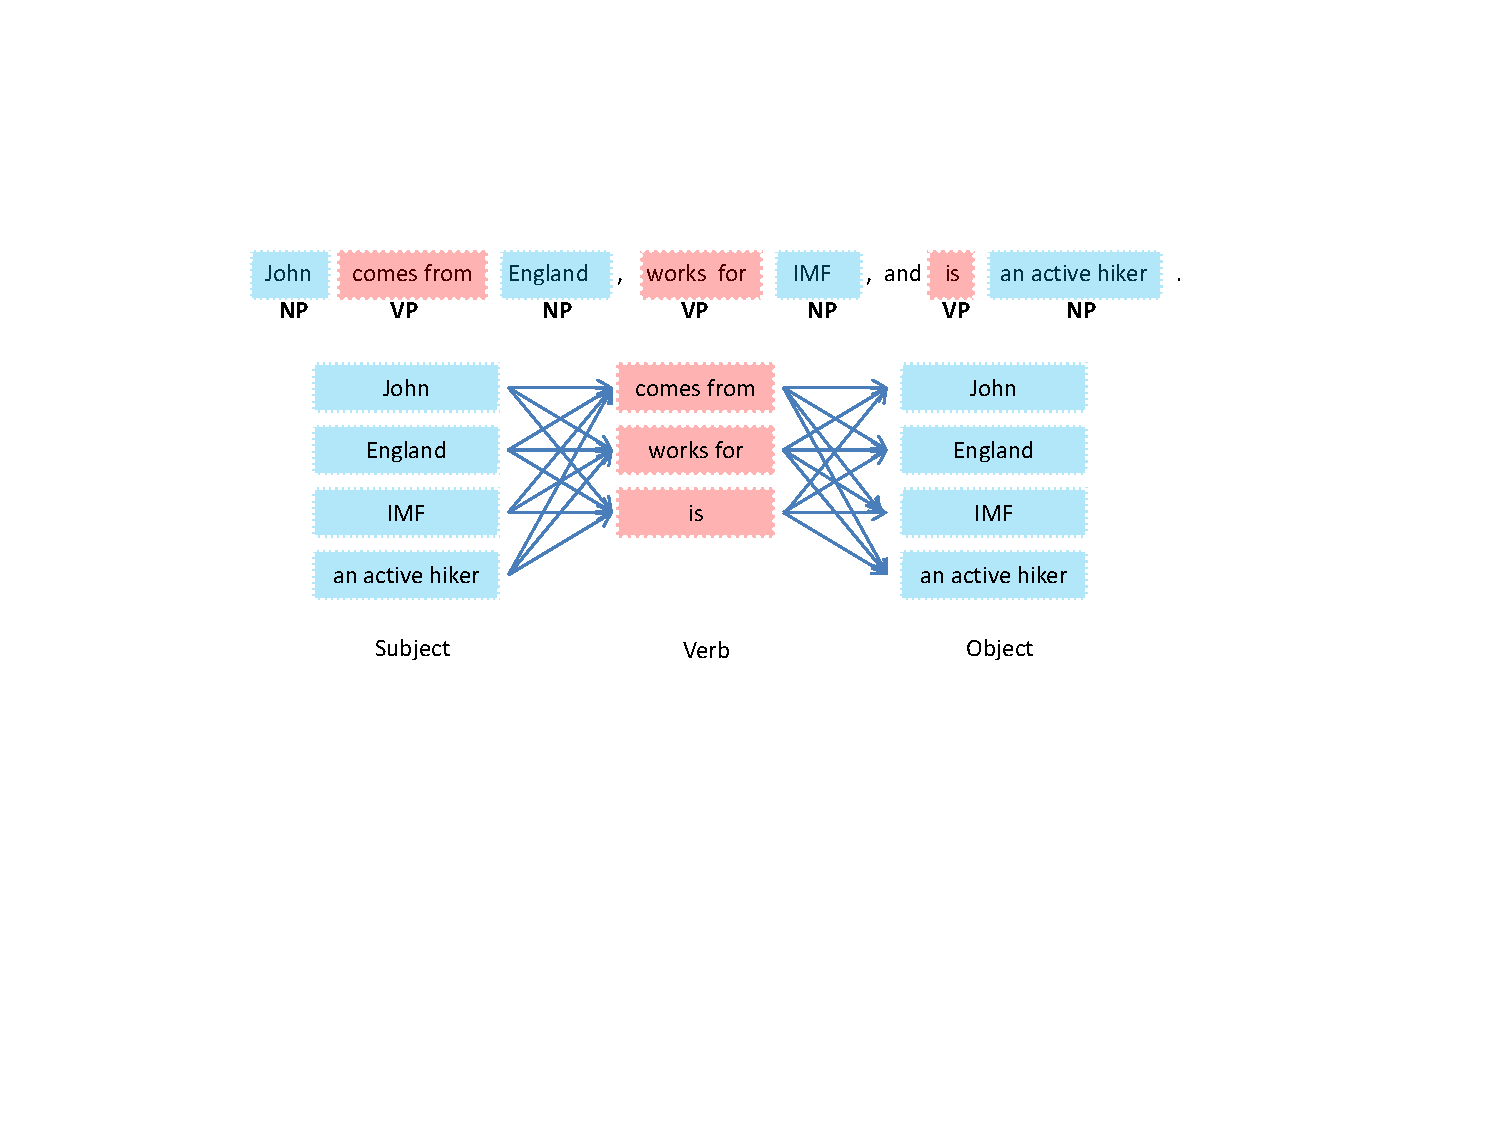
\includegraphics[scale=0.5]{figs/construct-simple-sents.pdf} 
	\caption{Constructing simple sentences}	
	\label{fig::ConstructSimpleSents}
\end{figure}


\subsection{Constructing simple sentences} 

We define a simple English sentence as a sentence with SVO structure, which has one subject, one verb and one object.
Our definition is similar to the definition of EAS, mentioned in section 1. 
However, we only focus on the SVO structure and other constraints are relaxed.
We assume both subjects (S) and objects (O) are noun phrases (NP) in the parse tree.
For a given English sentence $e$, we extract a list $S_{NP}$ of NPs and a list $S_V$ of verbs.
$S_{NP}$ has an additional empty NP in order to handle intransitive verbs.
A straightforward way to construct simple sentences is to enumerate all possible sentences based on $S_{NP}$ and $S_V$.
That results in $|S_{NP}|^2|S_V|$ simple sentences.

Figure~\ref{fig::ConstructSimpleSents} illustrates the constructions for ``\textit{John comes from England, works for IMF, and is an active hiker}''. 
The system extracts a noun phrase list $S_{NP}$ \{\textit{John, England, IMF, an active hiker}\} and a verb list $S_V$ \{\textit{comes from, works for, is}\}.
Our model constructs simple sentences such as ``\textit{John comes from England}'' , ``\textit{John comes from IMF}'' and ``\textit{John comes from an active hiker}''.
The total number of simple sentences, $|\mathbb{S}|$, is 48.

\subsection{Decoding algorithm} 

Given a list of simple sentences $\mathbb{S}$, the decoder's objective is to construct and find the best simplification candidate $\mathcal{S} \subset \mathbb{S}$.
We call $\mathcal{S}$ a \textit{hypothesis} in the context of the decoder.
The rationale behind our left-right stack decoding algorithm is to construct a hypothesis that covers all noun phrases and verb phrases of the original sentence.

The decoding task is to find the optimal solution over all possible combinations of simple sentences, given the feature values and learned feature weights.
Depending on the number of simple sentences per hypothesis, the search space grows exponentially.
Since each simple sentence contains an object, we can group the candidate sentences by the object noun phrase.
As a result, it is not necessary to evaluate all combinations; we can look at one object at a time from left to right.
Figure~\ref{fig::decode-by-object} demonstrates the idea of decoding via objects.
We have three objects ``\textit{England}'', ``\textit{IMF}'' and ``\textit{an active hiker}''.
The algorithm first finds potential simple sentences which have ``\textit{England}'' as object.
After finishing ``England'', the algorithm expands to ``\textit{IMF}'' and ``\textit{an active hiker}''.
In this example the optimal path is the path with bold arrows.

\begin{figure}[t]
	\centering
	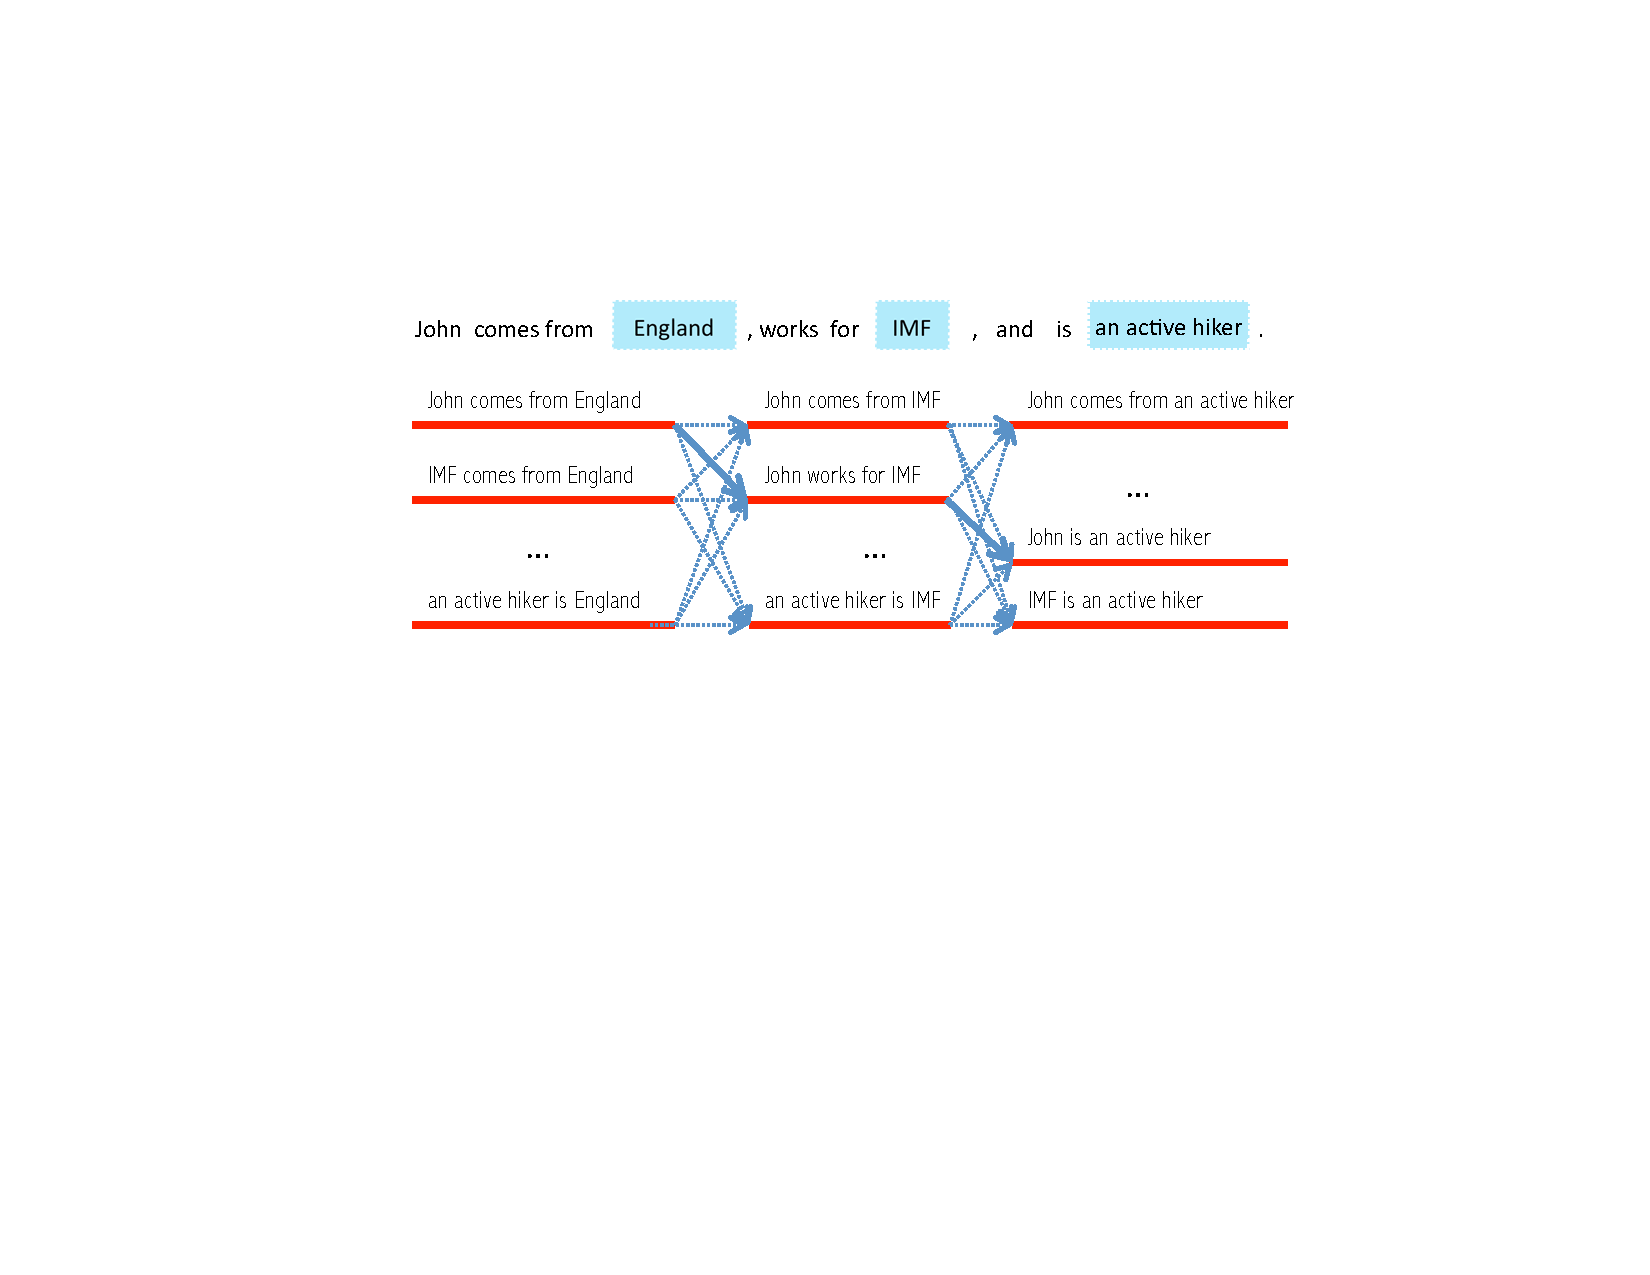
\includegraphics[width=75mm]{figs/decode-by-object.pdf} 	
	\caption{Left-right decoding by objects}
	\label{fig::decode-by-object}
\end{figure}


\begin{algorithm}
	\caption{: K-Best Stack Decoding}	
	\label{stack-decoding}
	\begin{algorithmic}[1]
		\STATE Initialize an empty hypothesis list \textit{HypList}
		\STATE Initialize \textit{HYPS} is a stack of 1-simple-sentence hypotheses

		\FOR{$i = 0$ to $|S_V|$}
			\STATE Initialize stack $expand_h$
			\WHILE{\textit{HYPS} is not empty} 				
				\STATE pop $h$ from \textit{HYPS}
				\STATE $expand_h$ $\gets$ Expand-Hypothesis($h$)
			\ENDWHILE
			\STATE $expand_h$ $\gets$ Prune-Hypothesis($expand_h$, \textit{stack-size})
			\STATE \textit{HYPS} $\gets$ $expand_h$			
			\STATE Store hypotheses of $expand_d$ into \textit{HypList}
		\ENDFOR
		
		\STATE \textit{SortedHypList} $\gets$ Sort-Hypothesis(\textit{HypList})
		
		\STATE Return K-best hypotheses in \textit{SortedHypList}
	\end{algorithmic}
\end{algorithm}

Algorithm \ref{stack-decoding} is a version of stack decoding for sentence simplification.
The decoding process advances by extending a state that is equivalent to a stack of hypotheses.
Line 1 and 2 initialize \textit{HYPS} stack and \textit{HypList}.
A \textit{HYPS} stack maintains a current search state, meanwhile \textit{HypList} stores potential hypotheses after each state.
\textit{HYPS} is initialized with hypotheses containing one simple sentence.
Line 3 starts a loop over states. 
The number of maximum states is equal to the size of $S_V$ plus one.
Lines 4-8 represent the hypothesis expansion.

\begin{figure}[ht]%
\centering
\subfloat[Pop and Expand]{ 
	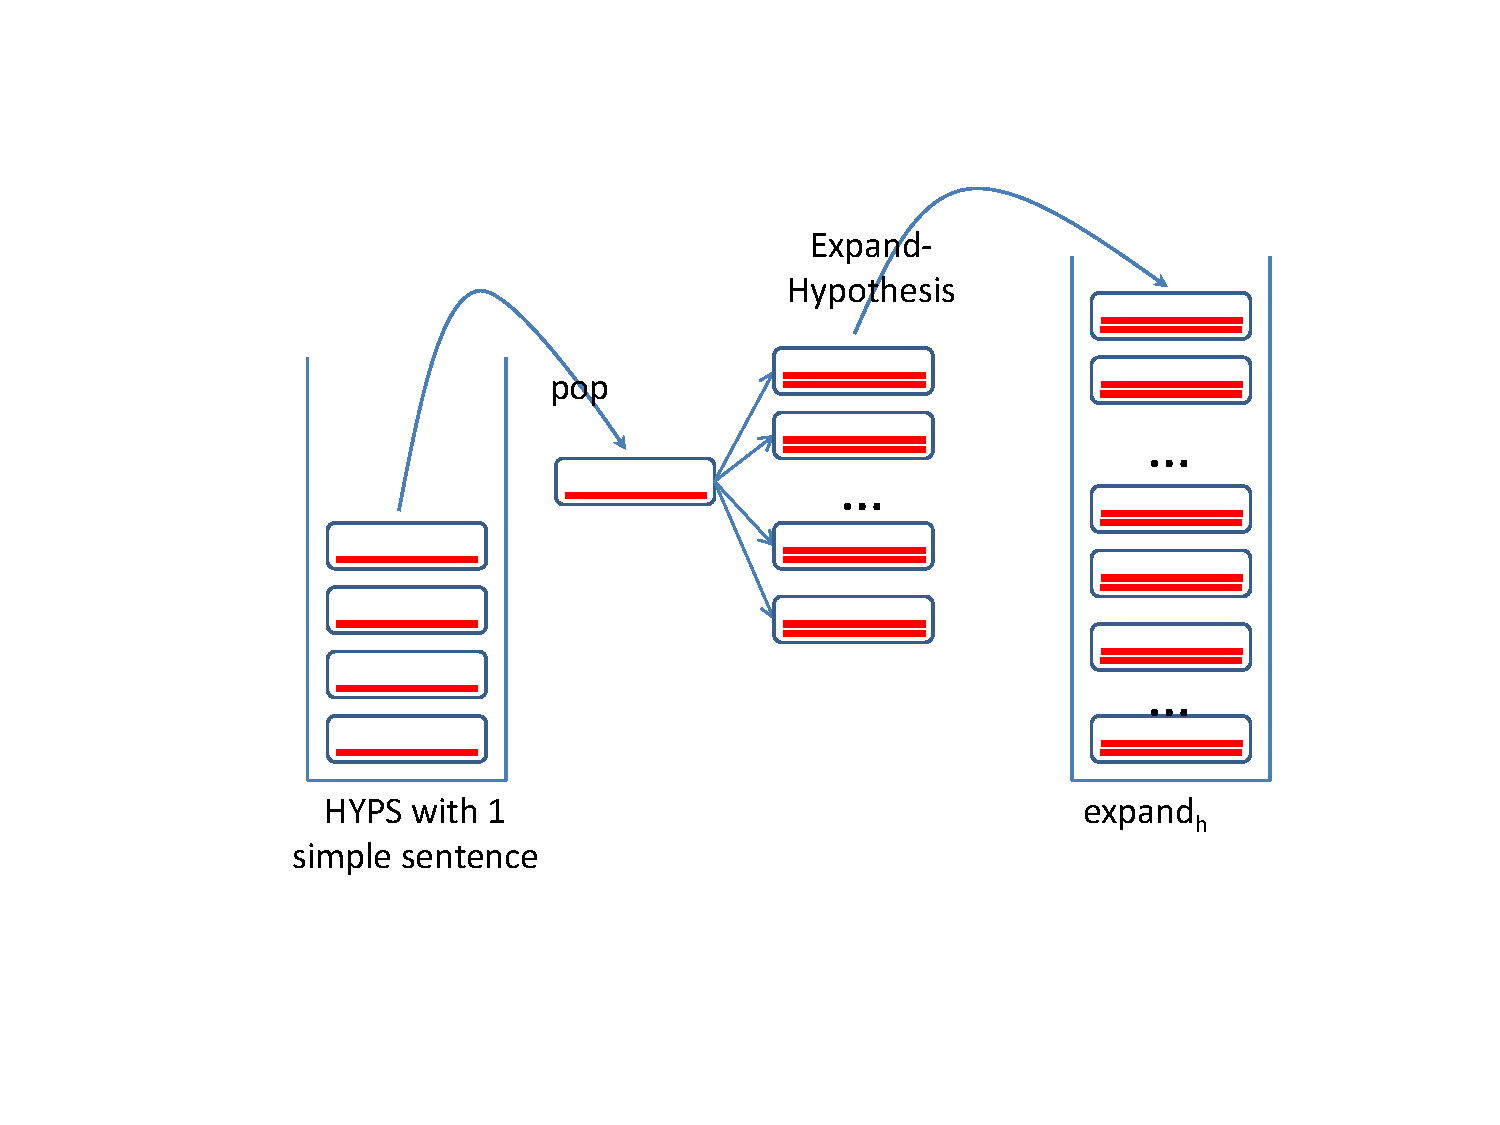
\includegraphics[height=45mm]{figs/stack-a.pdf} 
	\label{fig::expand}
}\\
\subfloat[Hypothesis pruning]{ 
	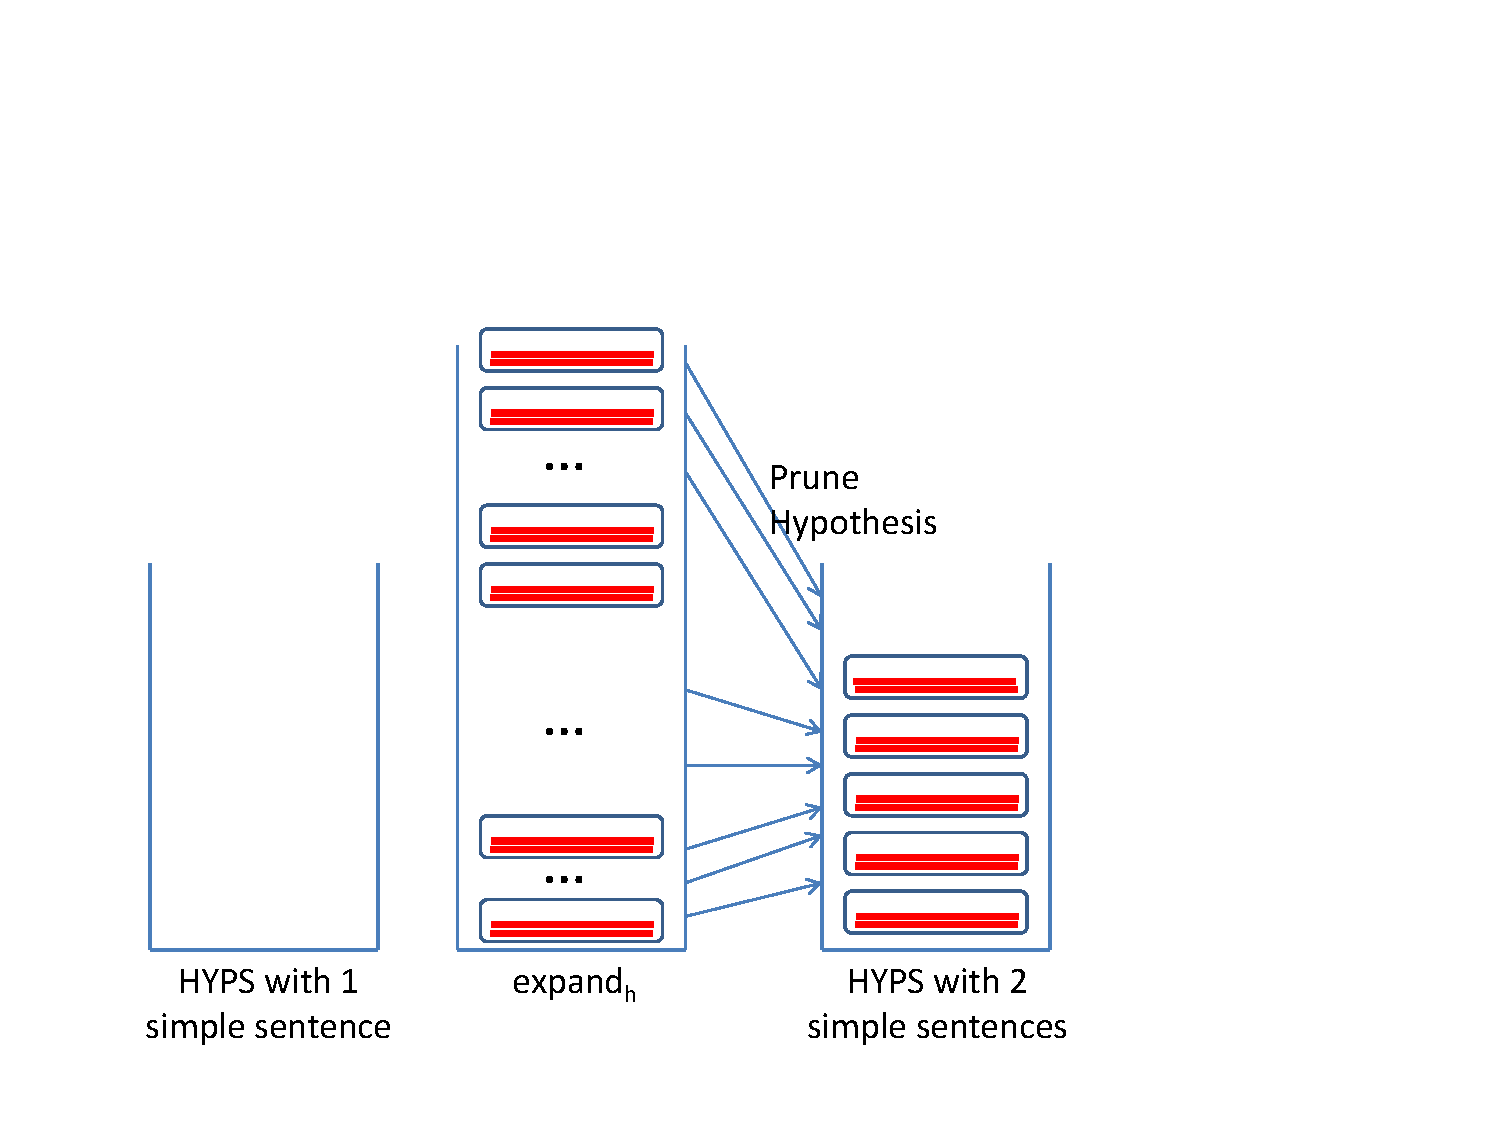
\includegraphics[height=45mm]{figs/stack-c.pdf}
	\label{fig::prune}
}
\caption{A visualization for stack decoding}
\end{figure}

Figure~\ref{fig::expand} illustrates the pop-expand process of \textit{HYPS} stack with 1-simple-sentence hypotheses.
The expansion in this situation expands to a 2-simple-sentence hypotheses-stack $expand_h$.
The size of $expand_h$ will exponentially increase according to the size of $S_V$ and $S_{NP}$.
Therefore, we prefer to maintain $expand_h$ within a limit number (\textit{stack-size}) of hypotheses.
Line 9 helps the decoder to control the size of $expand_h$ by applying different pruning strategies: word coverage, model score or both.
Figure~\ref{fig::prune} illustrates the pruning process on $expand_h$ with 2-simple-sentence hypotheses.
Line 10 replaces the current state with a new state of the expanded hypotheses.
Before moving to a new state, \textit{HypList} is used to preserve potential hypotheses of the current state.
Line 13 sorts hypotheses in \textit{HypList} according to their model scores and a K-best list is returned in line 14.

\section{Learning}
\label{sec:Learning}

Since defining a log-linear sentence simplification model and decoding algorithm has been completed, this section describes a discriminative learning algorithm for the \textit{learning problem}.
We learn optimized weight vector $w$ by using the Margin Infused Relaxed Algorithm or MIRA \cite{MIRA:2003}, which is an online learner closely related to both the support vector machine and perceptron learning framework.
In general, weights are updated at each step time $i$ according to:
\begin{equation}
\begin{array}{cc}
& w_{i+1}  = \arg\min_{w_{i+1}} ||w_{i+1} - w_i||   \\
\\
\mbox{s.t.} & score(\mathcal{S},e) \geq score(\mathcal{S}',e) + L(\mathcal{S},\mathcal{S}') 
\end{array}
\end{equation}
where $L(\mathcal{S},\mathcal{S}')$ is a measure of the loss of using $\mathcal{S}'$ instead of the simplification reference $\mathcal{S}$; $score()$ is a cost function of $e$ and $\mathcal{S}$ and in this case is the decoder score.

\begin{algorithm}
	\caption{: MIRA training for Sentence Simplifier}
	\label{algo:MIRA}
	\begin{algorithmic}
		\STATE training set $\tau=\{f_t, e_t\}_{t=1}^{T}$ has T original English sentences with the feature vector $f_t$ of $e_t$.
		\STATE $\varepsilon$ is the simplification reference set.
		\STATE m-oracle set $O = \{\}$.
		\STATE The current weight vector $w^i$. 
	\end{algorithmic}	
	
	\begin{algorithmic}[1]
		\STATE i=0		
		%loop over Q iterations
		\FOR{$j = 1$ to Q} 		
			%loop over T original English sentences
			\FOR {$t = 1$ to T} 
				%get k-best simplified candidates of sentence $e_t$
				\STATE $H$ $\gets$ get\_K\_Best($\mathcal{S}_t$ ; $w^i$)
				%get oracle list
				\STATE $O$ $\gets$ get\_m\_Oracle($H$ ; $\varepsilon_t$)
				\STATE $\gamma$ = $\sum\limits_{o=1}^m \sum\limits_{h=1}^{K} \alpha(e_o, e_h ; \varepsilon_t) (f_{e_o}  - f_{e_h})$
				\STATE $w^{i+1}$ = $w^i$ + $\gamma$
				
				\STATE $i = i + 1$
			\ENDFOR
		\ENDFOR
		\STATE Return $\frac{\sum_{i=1}^{Q*T} w^i}{Q*T}$
	\end{algorithmic}
\end{algorithm}

Algorithm~\ref{algo:MIRA} is a version of MIRA for training the weights of our sentence simplification model.
On each iteration, MIRA considers a single instance from the training set $(\mathcal{S}_t, e_t)$ and updates the weights so that the score of the correct simplification $\varepsilon_t$ is greater than the score of all other simplifications by a margin proportional to their loss.
However, given a sentence there are an exponential amount of possible simplification candidates.
Therefore, the optimizer has to deal with an exponentially large number of constraints.
To tackle this, we only consider $K$-best hypotheses and choose $m$-oracle hypotheses to support the weight update decision.
This idea is similar to the way MIRA has been used in dependency parsing and machine translation \cite{McDonald-et-al:2005,acl06:liang,watanabe-EtAl:2007:EMNLP-CoNLL}.

On each update, MIRA attempts to keep the new weight vector as close as possible to the old weight vector.
Subject to margin constraints keep the score of the correct output above the score of the guessed output by updating an amount given by the loss of the incorrect output.
In line 6, $\alpha$ can be interpreted as an update step size; when $\alpha$ is a large number we want to update our weights aggressively, otherwise weights are updated conservatively.
$\alpha$ is computed as follow:
\begin{equation}
\begin{array}{l}
\alpha = \max ( 0, \delta ) \\
\delta = \min \Bigg\lbrace C, \frac{ L(e_o, e_h ; \varepsilon_t) - [score(e_o) - score(e_h)] }{ ||\mathcal{S}_{e_o}  - f_{e_h}||_{2}^2}  \Bigg\rbrace \\
\end{array}
\label{equa:update}
\end{equation}
where 
$C$ is a positive constant used to cap the maximum possible value of $\alpha$; $score()$ is the decoder score; and $L(e_o, e_h ; \varepsilon_t)$ is the loss function.

$L(e_o, e_h ; \varepsilon_t)$ measures the difference between oracle $e_o$ and hypothesis $e_h$ according to the gold reference $\varepsilon_t$.
$L$ is crucial to guide the optimizer to learn optimized weights.
We defined $L(e_o, e_h ; \varepsilon_t)$ as follow
\begin{equation}
\begin{array}{l}
L(e_o, e_h ; \varepsilon_t) = AveF_N(e_o,\varepsilon_t) - AveF_N(e_h,\varepsilon_t) 
\end{array}
\end{equation}
where $AveF_N(e_o,\varepsilon_t)$ and $AveF_N(e_h,\varepsilon_t)$ is the average n-gram (n=[2:N]) cooccurrence F-score of $(e_o,\varepsilon_t)$ and $(e_h,\varepsilon_t)$, respectively.
In this case, we optimize the weights directly against the $AveF_N$ metric over the training data.
$AveF_N$ can be substituted by other evaluation metrics such as the ROUGE family metric \cite{lin-ROUGE:2004}.
Similar to the perceptron method, the actual weight vector during decoding is averaged across the number of iterations and training instances; and it is computed in line 11.

\section{Modeling}
\label{sec:Modeling}

We now turn to the \textit{modeling problem}.
Our fundamental question is: given the model in Equation~\ref{equ::model} with $M$ feature functions, what linguistic features can be leveraged to capture semantic information of the original sentence?
We address the question in this section by describing features that cover different levels of linguistic structures.
Our model incorporates 177 features based on information from the original English sentence $e$ which contains chunks, syntactic and dependency parse trees \cite{Ramshaw95,StanfordDepParser:2006}.

\subsection{Simple sentence level features}

A simplification hypothesis $s$ contains $k$ simple sentences.
Therefore, it is crucial that our model chooses reasonable simple sentences to form a hypothesis.
For each simple sentence $s_i$ we incorporated the following feature functions:

\textbf{Word Count\ \ \ } These features count the number word in subject (S), verb (V) and object (O), also counting the number of proper nouns in S and the number of proper nouns in O.

\textbf{Distance between NPs and Verbs\ \ \ } These features focus on the number of NPs and VPs in between S, V and O.
This feature group includes the number of NPs between S and V, the number of NPs between V and O,  the number of VPs between S and V, the number of VPs between V and O.

\textbf{Dependency Structures\ \ \ } It is possible that the decoder constructs semantically incorrect simple sentences, in which S, V, and O do not have any semantic connection.
One way to possibly reduce this kind of mistake is analyze the dependency chain between S, V, and O on the original dependency tree of $e$.
Our dependency structure features include the minimum and maximum distances of (S:O), (S:V), and (V:O). 

\textbf{Syntactic Structures\ \ \ } Another source of information is the syntactic parse tree of $e$, which can be used to extract syntactic features.
The sentence-like boundary feature considers the path from S to O along the syntactic parse tree to see whether it crosses the sentence-like boundary (e.g. relative clauses).
For example in the original sentence ``\textit{John comes from England and works for IMF which stands for International Monetary Funds}'', the simple sentence ``\textit{IMF stands for International Monetary Funds}'' has sentence-like boundary feature is triggered since the path from ``\textit{IMF}'' to ``\textit{International Monetary Funds}'' on the syntactic tree of the original sentence contains an SBAR node.

Another feature is the PP attachment feature.
This checks if the O contains a prepositional phrase attachment or not.
Moreover, the single pronoun feature will check if S and O are single pronoun or not.
The last feature is VO common ancestor, which looks at the syntactic tree to see whether or not V and O share the same VP tag as a common ancestor. 

\subsection{Interactive simple sentence features}

%A good simplification hypothesis not only contains good simple sentences $s_i$ but also has a good set of simple sentences $s$.
A collection of grammatically sound simplified sentences does not necessarily make a good hypothesis
Dropping words, unnecessary repetition, or even wrong order can make the hypothesis unreadable. 
Therefore, our model needs to be equipped with features that are capable to measure the interactiveness across simple sentences and are also able to represent $s$ in the best possible manner.
We incorporated the following features into our model:

\textbf{Sentence Count\ \ \ } This group of features consider the number of sentences in the hypothesis. It consists of an integral feature of sentence count $sci = |S|$, and a group of binary features $scb_k = \delta(|S|)=k$ where $k \in [1,6] $ is the number of sentence.

\textbf{NP and Verb Coverage\ \ \ } The decoder's objective is to improve the chance of generating hypotheses that cover all NP and verbs of the original sentence $e$.
These features count the number of NPs and verbs that have been covered by the hypothesis, by the 1st and 2nd simple sentences.
Similarly, these features also count the number of missing NPs and verbs.

\textbf{S and O cross sentences\ \ \ } These features count how many times S of the 1st simple sentence is repeated as S of the 2nd simple sentence in a hypothesis.
They also count the number of times O of the 1st sentence is the S of 2nd sentence.

\textbf{Readability\ \ \ } This group of features computes statistics related to readability.
It includes Flesch, Gunning-Fog, SMOG, Flesch-Kincaid, automatic readability index, and average all scores \cite{Flesch:1948,Gunning:1968,SMOG:1969,kincaid:1975}.
Also, we compute the edit-distance of hypothesis against the original sentence, and the average word per simple sentence.

\textbf{Typed Dependency\ \ \ } At simple sentence level we examine dependency chains of S, V and O, while at the hypothesis level we analyze the typed dependency between words.
Our model has 46 typed dependencies which are represented by the 92 count features for the 1st and 2nd simple sentence.

\section{Experiments and Analysis}
\label{sec:Experiments}

\subsection{Data}

To enable the study of sentence simplification with our statistical models, we search for \textit{parallel} corpora, in which the sources are original English sentences and the target is its simplification reference.
For example, the source is ``\textit{Lu is married to Lian Hsiang , who is also a vajra master , and is referred as Grand Madam Lu }''.
The simplification reference contains 3 simple sentences which are ``\textit{Lu is married to Lian Hsiang}''; ``\textit{Lian Hsiang is also a vajra master}''; 
``\textit{Lu is referred as Grand Madam Lu}''. 
To the best of our knowledge, there is no such publicly available corpora under these conditions\footnote{We are aware of data sets from \cite{CohnLapata:2008,Zhu:2010}, however, they are more suitable in sentence compression task than in our task.}.

Our first attempt is to collect data automatically from original English and Simple English Wikipedia, based on the suggestions of Napoles and Dredze \shortcite{napoles-dredze:2010:CLW}.
However, we found that the collected corpus is unsuitable for our model. 
For example, consider the original sentence ``\textit{Hawking was the Lucasian Professor of Mathematics at the University of Cambridge for thirty years, taking up the post in 1979 and retiring on 1 October 2009}''.
The Simple Wikipedia reads ``\textit{Hawking was a professor of mathematics at the University of Cambridge (a position that Isaac Newton once had)}'' and ``\textit{He retired on October 1st 2009}''.
The problems with this are that ``\textit{(a position that Isaac Newton once had)}'' did not appear in the original text, and the pronoun ``\textit{He}'' requires our model to perform anaphora resolution which is out of scope of this work.

We finally decided to collect a set of sentences for which we obtained one manual simplification per sentence.
The corpus contains 854 sentences, among which 25\% sentences are from the New York Times and 75\% sentences are from Wikipedia. 
The average sentence length is 30.5 words.
We reserved 100 sentences for the unseen test set and the rest is for the development set and training data.
The annotators were given instructions that explained the task and defined sentence simplification with the aid of examples.
They were encouraged not to introduce new words and try to simplify by restructuring the original sentence.
They were asked to simplify while preserving all important information and ensuring the simplification sentences remained grammatically correct\footnote{Our corpus will be made publicly available for other researchers.}. 
Some examples from our corpus are given below:\\

\noindent Original: ``\textit{His name literally means Peach Taro ; as Taro is a common Japanese boy 's name , it is often translated as Peach Boy .}''\\ 
Simplification: ``\textit{His name literally means Peach Taro}'' ; ``\textit{Taro is a common Japanese boy 's name}'' ; ``\textit{Taro is often translated as Peach Boy}''\\

\noindent Original: ``\textit{These rankings are likely to change thanks to one player , Nokia , which has seen its market share shrink in the United States .}''\\
Simplification: ``\textit{These rankings are likely to change thanks to one player , Nokia}'' ; ``\textit{Nokia has seen its market share shrink in the United States}''

\subsection{Evaluation methods}

%{\bf QIN: From a reviewer's perspective, I may attach like this: You only evaluate on 100 sentences, why not do a human evaluation? How many top-best is grammatical and how many are really simplified?}
Evaluating sentence simplification is a difficult problem.
One possible way to overcome this is to use readability tests.
There have been readability tests such as Flesch, Gunning-Fog, SMOG, Flesch-Kincaid, etc. \cite{Flesch:1948,Gunning:1968,SMOG:1969,kincaid:1975}. 
In this work, we will use Flesch-Kincaid grade level which can be interpret as the number of years of education generally required to understand a text.

Furthermore, automatic evaluation of summaries has also been explored recently.
The work of Lin \shortcite{lin-ROUGE:2004} on the ROUGE family metric is perhaps the best known study of automatic summarization evaluation.
Other methods have been proposed such as Pyramid \cite{Nenkova-et-al:2007}.
Recently, Aluisio et al. \shortcite{Aluisio-et-al:2010} proposed readability assessment for sentence simplification. 

Our models are optimized toward $AveF_{10}$, which is the average F-score of $n$-gram concurrence between hypothesis and reference in which $n$ is from 2 to 10.
Besides $AveF_{10}$, we will report automatic evaluation scores on the unseen test set in Flesch-Kincaid grade level, ROUGE-2 and ROUGE-4. 
When we evaluate on a test set, a score will be reported as the average score per sentence.

\subsection{Model behaviors}

\begin{figure*}[ht]%
	\centering
	\subfloat[\textit{stack-size}]{ 
		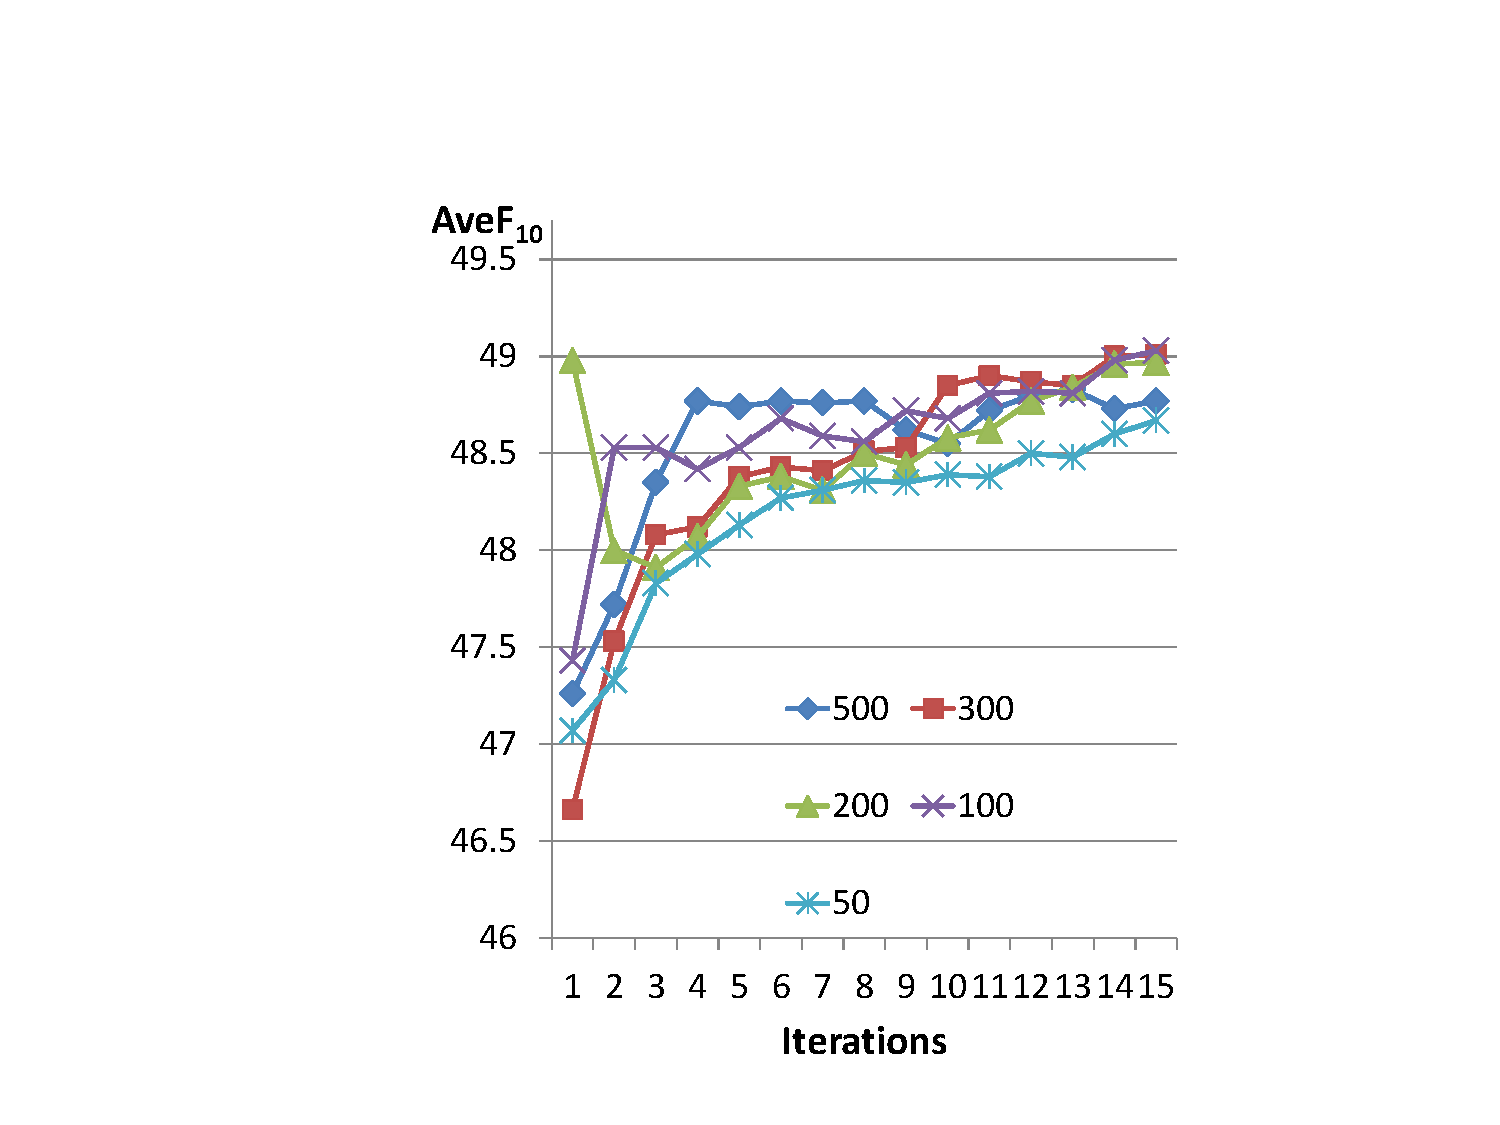
\includegraphics[width=38mm]{figs/max-stack-size.pdf} 
		\label{fig:stack-size}
	}
	\subfloat[K-best]{ 
		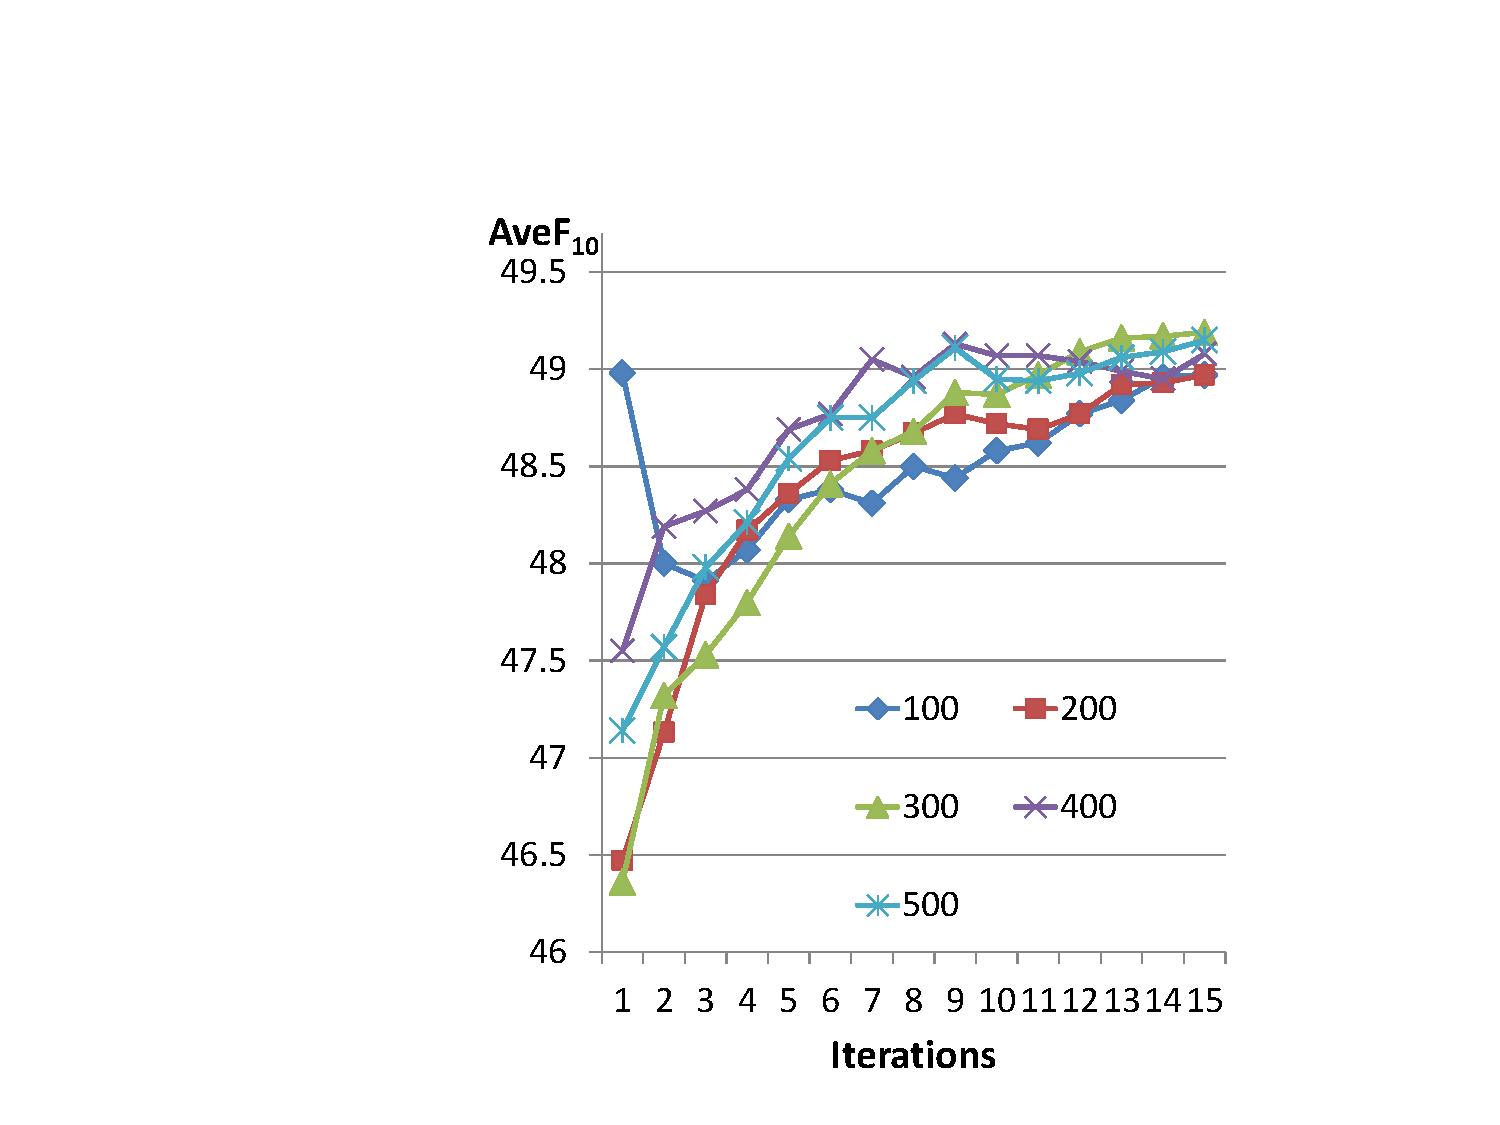
\includegraphics[width=38mm]{figs/k-best-size.pdf}  
		\label{fig:k-best}
	}
	\subfloat[Constant C]{ 
		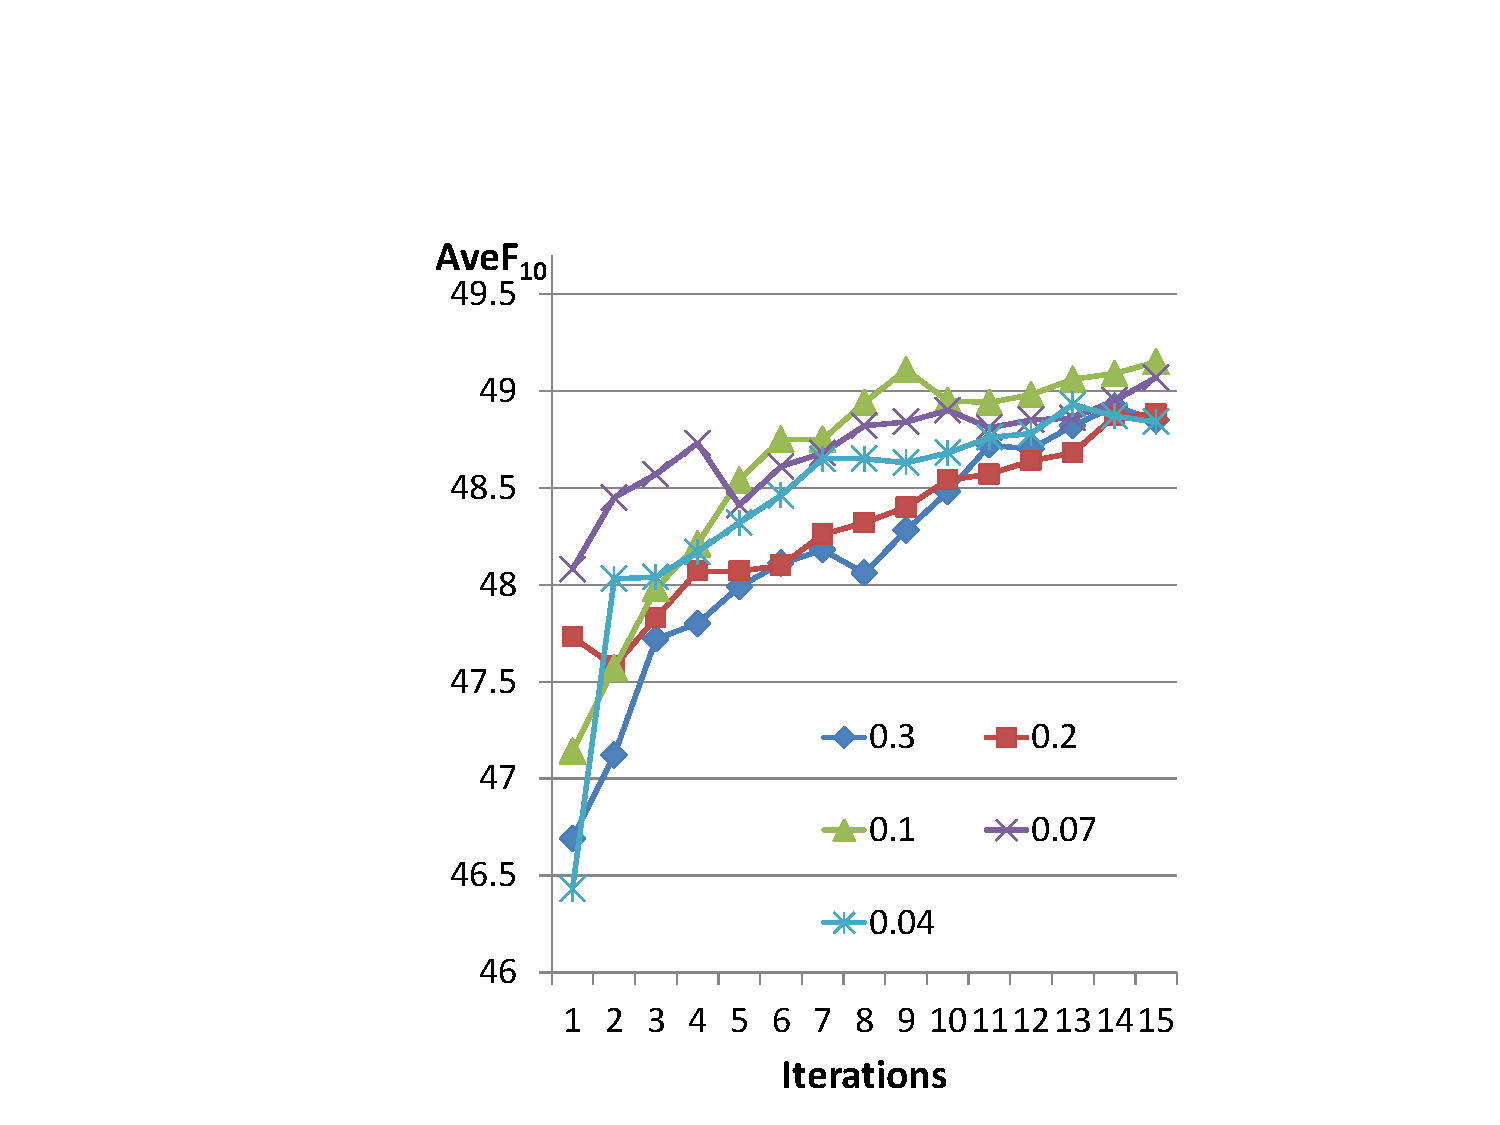
\includegraphics[width=38mm]{figs/constant-C.pdf}  
		\label{fig:constant-C}
	}
	\subfloat[m-oracle]{ 
		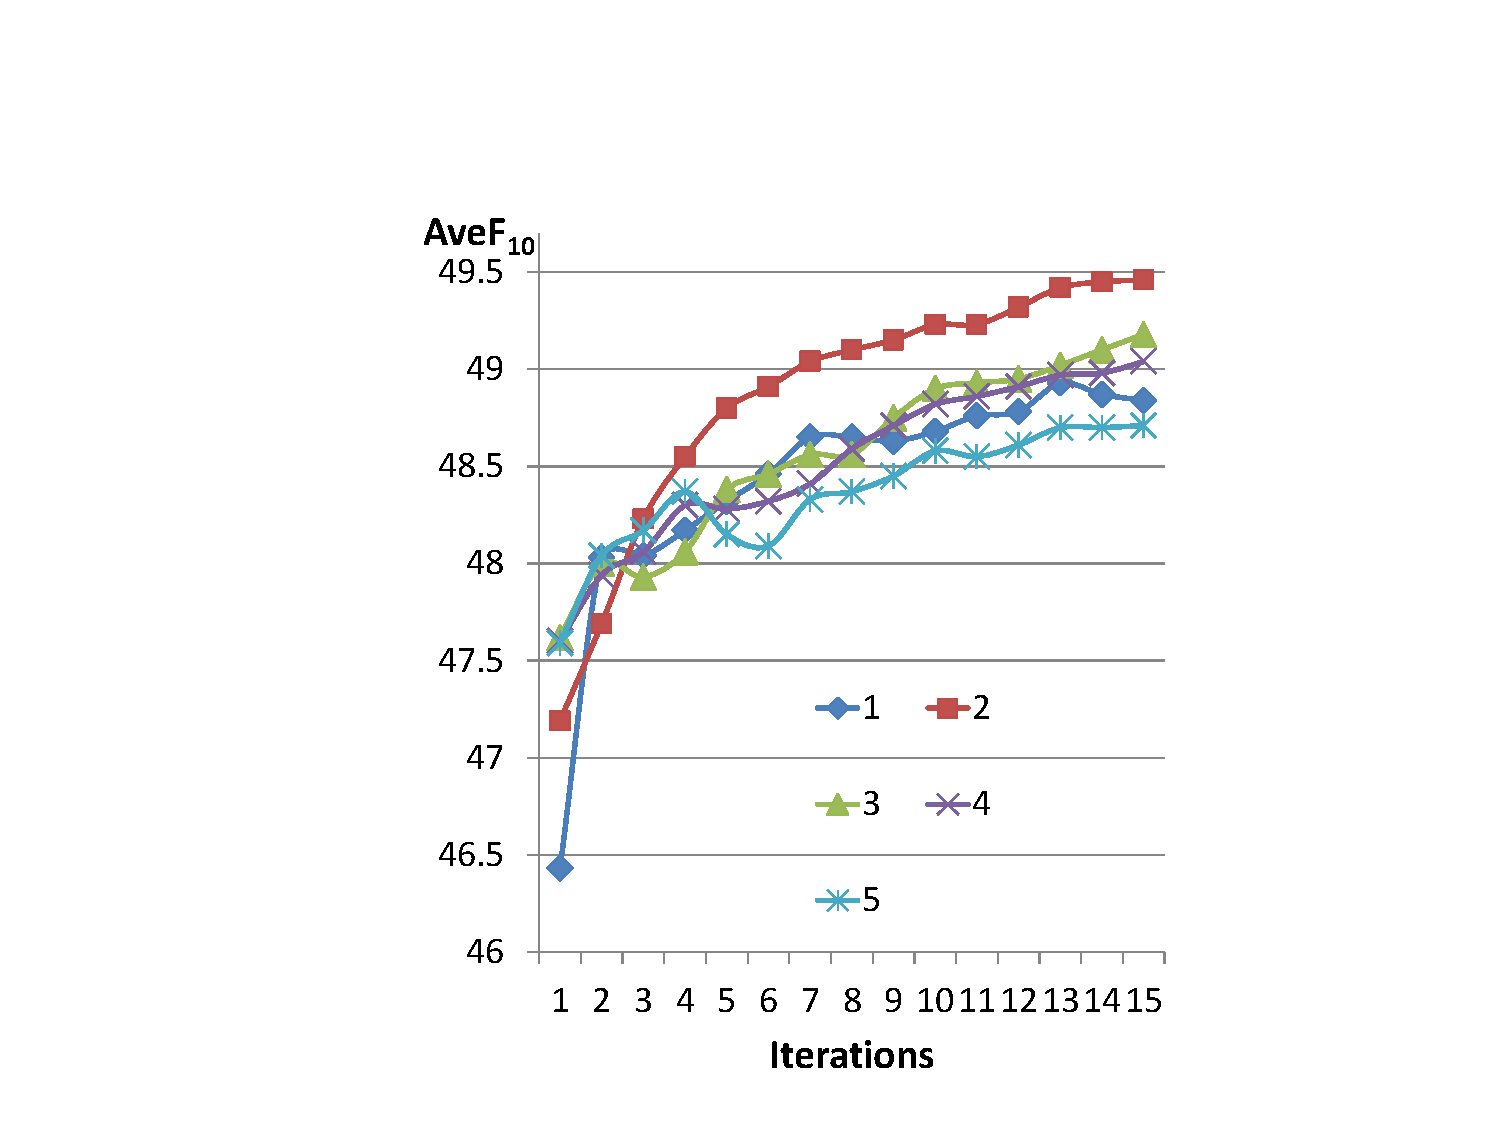
\includegraphics[width=38mm]{figs/m-oracle.pdf}  
		\label{fig:m-oracle}
	}
\caption{Performance of the sentence simplifier on training data over 15 iterations when optimized toward $AveF_{10}$ metric and under various conditions.}
\label{fig::fscore}
\end{figure*}


How well does our system learn from the labeled corpus?
To answer this question we investigate the interactions of model and decoder hyper parameters over the training data.
We performed controlled experiments on \textit{stack-size}, K-best, C, and m-oracle parameters.
For each parameter, all other model and decoder values are fixed, and the only change is with the parameter's value of interest.
Figure~\ref{fig::fscore} illustrates these experiments with parameters over the training data during 15 MIRA training iterations with $AveF_{10}$ metric.
The weight vector $w$ is initialized randomly.

In Figure~\ref{fig:stack-size}, we experimented with 5 different values from 100 to 500 hypotheses per stack. 
The expected outcome is when we use a larger \textit{stack-size} the decoder may has more chance to find better hypotheses.
However, a larger \textit{stack-size} will obviously cost more memory and run time is slower.
Therefore, we want to find a \textit{stack-size} that compromises conditions.
These experiments show that with a \textit{stack-size} of 200, our model performed reasonably well in comparison with 300 and 500.
A \textit{stack-size} of 100 is no better than 200, while a \textit{stack-size} of 50 is much worse than 200.

In Figure~\ref{fig:k-best}, we experimented with 5 different values of K-best list with K from 100 to 500.
We observed a K-best list of 300 hypotheses seems to perform well compare to other values.
In terms of stability, the curve of 300-best list appears less fluctuation than other curves over 15 iterations.

C is the hyper-parameter which is used in Equation~\ref{equa:update} for weight updating in MIRA.
Figure~\ref{fig:constant-C} shows experiments with different constant C.
If C is a large number, it means our model prefers an aggressive weight updating scheme, otherwise, our model updates weights conservatively.
When C is 0.3 or 0.2 the performance is worse than 0.1 or 0.07 and 0.04.

The last controlled experiments are shown in Figure~\ref{fig:m-oracle}, in which we test different values of $m$ ranging from 1 to 5.
These experiments show that using 2 oracle hypotheses consistently leads to better performances in comparison with other values.

\subsection{Performance on the unseen test set}

After exploring different model configurations we trained the final model with \textit{stack-size} = 200; K-best = 300; C = 0.04; and m-oracle = 2.
$AveF_{10}$ score of the final system on the training set is 50.69 which is about one $AveF_{10}$ point better than any system in Figure~\ref{fig::fscore}.
We use the final system to evaluate on the unseen test set.
Also, we compare our system with the rule-based system (henceforth H\&S) proposed by Heilman and Smith \shortcite{HeilmanSmith:2010}.%
\footnote{We thank Michael Heilman for providing us his code.}\footnote{We could not reach the authors of \cite{Zhu:2010} in order to obtain outputs. Kristian Woodsend kindly provided us \textbf{partial outputs} of \cite{woodsend-lapata:2011:EMNLP}, therefore we did not include their outputs in this section.}

\begin{table}[h]
\begin{center}
\begin{tabular}{cccc}\toprule
Original & Reference & H\&S & Our system\\ 
9.6 & 8.2 & 8.3 & 7.9 \\ 
\bottomrule
\end{tabular} 
\end{center}
\caption{Flesch-Kincaid grade level of original, reference, H\&S, and our proposed simplification on the unseen test set.}
\label{table::Flesch-Kincaid}
\end{table}

\begin{table}[h]
\begin{center}
\begin{tabular}{cccc}\toprule
System & $AveF_{10}$ & ROUGE-2 & ROUGE-4 \\ 
\midrule
H\&S & 51.0 & 82.2 &  72.3\\
Our system & 55.5 & 82.4 & 72.9 \\ 
\bottomrule
\end{tabular} 
\end{center}
\caption{Results on the unseen test set with $AveF_{10}$, ROUGE-2 and ROUGE-4 scores. Our system outperforms the rule-based system proposed by Heilman and Smith \shortcite{HeilmanSmith:2010}.}
\label{table::Others}
\end{table}

\begin{table*}[ht]
\begin{tiny}
\begin{center}
\begin{tabular}{p{2mm}p{149mm}}\toprule
\multicolumn{2}{c}{\textbf{Positive examples}} \\
O       & In 2011 , IBM gained worldwide attention for its artificial intelligence program Watson , which was exhibited on Jeopardy against game show champions Ken Jennings and Brad Rutter .\\ 
S       & Watson was exhibited on Jeopardy against game show champions Ken Jennings and Brad Rutter .\\
        & In 2011 , IBM gained worldwide attention for its artificial intelligence program Watson .\\               
R       & In 2011 , IBM gained worldwide attention for its artificial intelligence program Watson .\\
        & Watson was exhibited on Jeopardy against game show champions Ken Jennings and Brad Rutter .\\
\midrule
O       & He told Radiozurnal that he was halting the campaign for Christmas and would restart it in the new year .\\ 
S       & He told Radiozurnal .\\
        & He was halting the campaign for Christmas .\\
        & He would restart it in the new year .\\
R       & He told Radiozurnal .\\
        & He was halting the campaign for Christmas .\\
        & He would restart it in the new year .\\
\toprule
\multicolumn{2}{c}{\textbf{Negative examples}} \\
O       & He drives a 10-year-old Opel Corsa , but lives in a pleasant town house in the sleepy capital, Maseru, with wireless Internet and a housekeeper who comes twice a week .\\ 
S       & He drives a 10-year-old Opel Corsa .\\
        & He lives in a pleasant town house in the sleepy capital, Maseru, with wireless Internet and a housekeeper who .\\
R       & He drives a 10-year-old Opel Corsa .\\
        & He lives in a pleasant town house in the sleepy capital, Maseru, with wireless Internet and a housekeeper .\\
        & a housekeeper comes twice a week .\\
\midrule
O       &  An elderly Georgian woman was scavenging for copper to sell as scrap when she accidentally sliced through an underground cable and cut off Internet services to all of neighbouring Armenia , it emerged on Wednesday .\\
S       & An elderly Georgian woman was scavenging for copper to sell .\\
        & scrap cut off Internet services to all of neighbouring Armenia .\\
R       & An elderly Georgian woman was scavenging for copper to sell as scrap .\\
        & she accidentally sliced through an underground cable .\\
        & she cut off Internet services to all of neighbouring Armenia .\\
        & it emerged on Wednesday .\\
        
\bottomrule
\end{tabular} 
\end{center}
\caption{We show the original sentence (O), our simplification (S), and simplification reference (R). Positive examples are cases when our simplifications closely match with the reference. Meanwhile, negative examples show cases when our model can not produce good simplifications.}
\label{table::Examples}
\end{tiny}
\end{table*}



We first compare our system with H\&S in the Flesch-Kincaid grade level, which indicates comprehension difficulty when reading an English text.
The higher the number the more difficult the text.
Table~\ref{table::Flesch-Kincaid} shows the original text requires a reader of grade level 9 or 10.
Both H\&S and us provided simplification candidates, which are easier to read compared to the original text.
Our model generated simpler hypotheses than the reference, while H\&S outputs were slightly more difficult to read than the reference.


Next, we compare our system with H\&S in ngram-based metrics such as $AveF_{10}$, ROUGE-2 and ROUGE-4 as shown in Table~\ref{table::Others}.
Our results are better than H\&S by 0.2 and 0.6 point in ROUGE-2 and ROUGE-4, respectively.
More interestingly, our system outperformed H\&S by 4.5 points in $AveF_{10}$, which is a metric considering both precision and recall up to 10-gram.
Over 100 sentences of the unseen test set, H\&S outperforms us in 43 sentences, but is worse than our system in 51 sentences. 

Table~\ref{table::Examples} shows examples of our system on the unseen test set. 
We present examples in cases where the proposed model works well and does not work well.


%{\bf QIN: Although all the experiments do proof something about the model, but none of them answer the question: does it really work. To proof that, you need to give the number: how many hypotheses is acceptable by human judge. }

\subsection{Discussions}

This work shares the same line of research with \cite{Klebanov:2004,HeilmanSmith:2010} in which we all focus on sentence-level factual simplification.
However, a major focus of our work is on log-linear models which offer a new perspective for sentence simplification on decoding, training, and modeling problems.
To contrast, consider rule-based systems \cite{Klebanov:2004,Daelemans-et-al:2004,Siddharthan:2006,HeilmanSmith:2010}, in which sentence simplification processes are driven by hand-written linguistic rules. 
The linguistic rules represent prior information about how each word and phrase can be restructured.
In our model, each linguistic rule is encoded as a feature function and we allow the model to learn the optimized feature weights based on the nature of training data.

A potential issue is the proposed model might be susceptible to the sparseness issue. 
We alleviated this issue by using structure level and count feature functions which are lexically independent. 

There are some limitations in this work.
First, the proposed model does not introduce new words which may lead to generate grammatically incorrect simple sentences.
Second, we focus on structure simplification and not on lexical simplification.
Finally, the proposed model does not deal with anaphora resolution, which means our model can generate repeatedly noun phrases repeatedly in multiple simple sentences.

\section{Conclusions}
\label{sec:Conclusion}

In this paper we proposed a novel method for sentence simplification based on log-linear models.
Our major contributions are the stack decoding algorithm, the discriminative training algorithm, and the 177 feature functions within the model.
We have presented insight the analyses of our model in controlled settings to show the impact of different model hyper parameters.
We demonstrated that the proposed model outperforms a state-of-the-art rule-based system on ROUGE-2, ROUGE-4, and $AveF_{10}$ by 0.2, 0.6, and 4.5 points, respectively.

Another way to improve our model is feature engineering, which can be applied in future work.
To address the data sparsity issue, we plan to use crowd-sourcing such as Amazon Mechanical Turk to collect more training data.
We plan to incorporate an n-gram LM to improve the grammaticality of hypotheses.

\section*{Acknowledgements}

We would like to thank Colin Cherry for fruitful discussions and anonymous reviewers for helpful comments.
We also thank Julianne Mentzer for proofreading the final version of the paper. 
%\bibliographystyle{acl}
% you bib file should really go here
%\bibliography{ijcnlp2011}

\bibliographystyle{acl2010}
% you bib file should really go here 
%\bibliography{acl2010}
\begin{small}
\bibliography{smt_all}
\end{small}

\end{document}
